\documentclass{standalone}
\usepackage{tikz}
\usepackage{ctex,siunitx}
\usepackage{tkz-euclide}
\usepackage{amsmath}
\usetikzlibrary{patterns, calc}
\usetikzlibrary {decorations.pathmorphing, decorations.pathreplacing, decorations.shapes,}
\begin{document}
\small
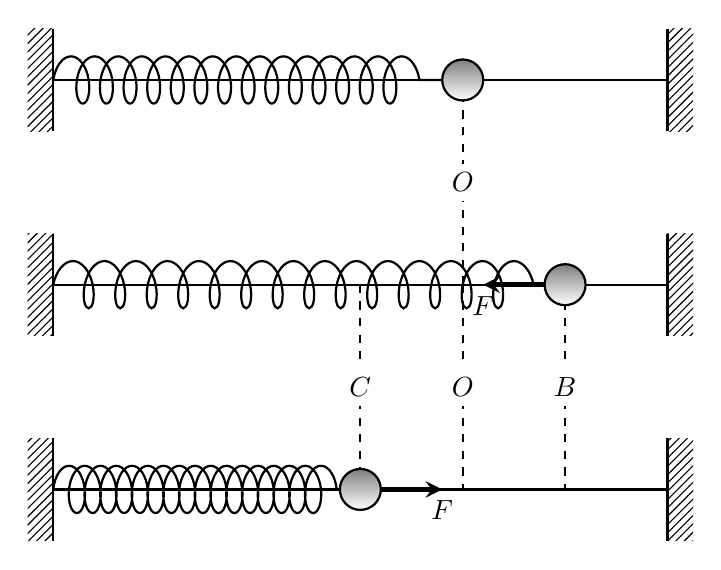
\begin{tikzpicture}[>=stealth,thick,scale=1.3]
  \tikzstyle{spring1}=[decorate,decoration={aspect=0.5, segment length=4mm, amplitude=3mm,coil}]
  \tikzstyle{spring2}=[decorate,decoration={aspect=0.5, segment length=3mm, amplitude=3mm,coil}]
  \tikzstyle{spring3}=[decorate,decoration={aspect=0.5, segment length=2mm, amplitude=3mm,coil}]
  \fill [pattern = north east lines] (-.25,2) rectangle (0,3);
  \fill [pattern = north east lines] (6,2) rectangle (6.25,3);
  \fill [pattern = north east lines] (-.25,0) rectangle (0,1);
  \fill [pattern = north east lines] (6,0) rectangle (6.25,1);
  \fill [pattern = north east lines] (-.25,-1) rectangle (0,-2);
  \fill [pattern = north east lines] (6,-1) rectangle (6.25,-2);
  \draw(0,2)--(0,3);  \draw(0,0)--(0,1);  \draw(0,-1)--(0,-2);
  \draw(6,2)--(6,3);  \draw(6,0)--(6,1);  \draw(6,-1)--(6,-2);
  \draw(0,2.5)--(6,2.5); \draw(0,.5)--(6,.5); \draw(0,-1.5)--(6,-1.5);
  \draw [->, ultra thick](5,.5)--(4.2,.5)node [below]{$F$};
  \draw [->, ultra thick](3,-1.5)--(3.8,-1.5)node [below]{$F$};
  \draw [dashed] (3, .5)--node [fill=white]{$C$}(3,-1.5);
  \draw [dashed] (4, .5)--node [fill=white]{$O$}(4,-1.5);
  \draw [dashed] (4, .5)--node [fill=white]{$O$}(4,2.5);
  \draw [dashed] (5, .5)--node [fill=white]{$B$}(5,-1.5);
  \draw [shade] (4, 2.5) circle(.2);
  \draw [shade] (5,.5) circle(.2);
  \draw [shade] (3,-1.5) circle(.2);
  \draw [spring2](0,2.5)--(4-.2,2.5);
  \draw [spring1](0,.5)--(5-.2,.5);
  \draw [spring3](0,-1.5)--(3-.2,-1.5);
\end{tikzpicture}
\end{document}